\section{Widzenie przez ściany (Bartosz Strzelecki)}

Do umiejętności wykorzystywanych przez gracza będzie należeć zdolność widzenia przeciwników oraz innych istotnych obiektów przez przeszkody.
Gracz po wciśnięciu przycisku przez krótki okres będzie w stanie zobaczyć sylwetki przeciwników znajdującymi się w jego polu widzenia.
Rozwiązanie jest inspirowane wcześniej wspomnianą grą Dead by Daylight (por. \ref{chap:dbd}). Markery nie poruszają się za celem lecz pojawiają się i pozostają w tym samym miejscu przez czas trwania animacji.

\begin{figure}[h]
\centering
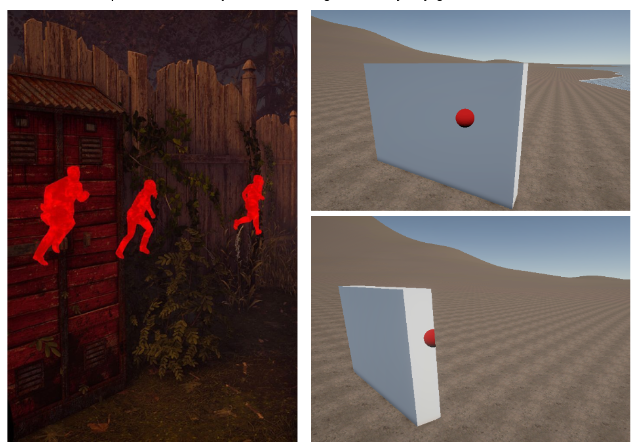
\includegraphics[width=0.6\textwidth]{images/shader}
\caption{Po lewej stronie przykład z gry Dead by Daylight. Po prawej zachowanie shadera w przypadku przysłanianiu markera przez przeszkody.}
\end{figure}

